%
%  Erik Olsen
%
\documentclass[12pt,fullpage]{article}
\usepackage{fullpage}                                        % use all of the page for text 
\usepackage{psfrag}                                          % LaTeX graphics tool
\usepackage{pslatex}                                         % avoids the default cmr font
\usepackage{graphicx}                                        % graphics package 
\usepackage{epsfig}                                          % figures
\usepackage{epsfig} 
\usepackage{hyperref}
\usepackage{color}

\begin{document}

\noindent
{\bf Rectangular distribution} (from \color{blue}\url{http://www.math.wm.edu/~leemis/chart/UDR/UDR.html}\color{black})

\noindent
The shorthand $X \sim$ rectangular$(n)$ is used to indicate that the
random variable $X$ has the rectangular distribution with positive parameter~$n$.
A rectangular random variable $X$ for some positive integer~$n$ has probability mass function 
$$
f(x) = \frac{1}{n + 1} \qquad \qquad x = 0,\, 1,\, 2, \ldots,\,n.
$$
The probability mass function with $n = 5$ is illustrated below.
{\begin{figure}[h!]
\begin{center}
\psfrag{labx}{$x$}
\psfrag{labf}{$f(x)$}
\psfrag{labff}{$1/6$}
\includegraphics[width=3.2in]{RectangularPlot.ps}
\end{center}
\end{figure}}

\noindent
The cumulative distribution function on
the support of $X$ is
$$
F(x) = \frac{x + 1}{n + 1} \qquad \qquad x = 0,\, 1,\, 2, \ldots,\,n.
$$
The survivor function on the support of $X$ is
$$
S(x) = P(X \ge x) = \frac{n + 1 - x}{n + 1}\qquad \qquad x = 0,\, 1,\, 2, \ldots,\,n.
$$
The hazard function on the support of $X$ is
$$
h(x) = \frac{f(x)} {S(x)}= \frac{1}{n + 1 - x} \qquad \qquad x = 0,\, 1,\, 2, \ldots,\,n.
$$
The cumulative hazard function on the support of $X$ is
$$
H(x) =  -\ln  \kern 0.04em S(x)= -\ln \left( \frac{n + 1 - x}{n + 1} \right) \qquad \qquad x = 0,\, 1,\, 2, \ldots,\,n.
$$
The inverse distribution function of $X$ is
$$
F^{-1}(u) = \lfloor (n + 1) u \rfloor \qquad \qquad 0 < u < 1.
$$
The median of $X$ is
$$
\frac{n-1}{2},
$$
when $n$ is even.\\
\\
The moment generating function of $X$ is 
$$
M(t) = E \left[e ^  {\kern 0.04em tx}\right] = \left\{ \begin{array}{ll}
       1 & \qquad t = 0 \\
       \frac{e ^ { {\kern 0.04em t (n + 1)}} - 1}{\left(e ^  {\kern 0.04em t} - 1 \right)(n + 1)} & \qquad t  \ne 0.
       \end{array} \right. 
$$
The characteristic function of X is
$$
\phi(t) = E \left[e ^  {\kern 0.04em itx}\right] = \left\{ \begin{array}{ll}
       1 & \qquad t = 0 \\
       \frac{e ^ { {\kern 0.04em it (n + 1)}} - 1}{\left(e ^  {\kern 0.04em it} - 1 \right)(n + 1)} & \qquad t \ne 0.
       \end{array} \right. 
$$
The population mean and variance of $X$ are
$$
E[X]=\frac{n}{2}\qquad \qquad
V[X]=\frac{n(n+2)}{12}.
$$
The skewness and kurtosis of $X$ are
$$
E\left[\left(\frac{X - \mu}{\sigma}\right) ^ {\kern -0.08 em 3} \right] = 0 \qquad \qquad
E\left[\left(\frac{X - \mu}{\sigma}\right) ^ {\kern -0.08 em 4} \right] = \frac{3}{5}\,\cdot \frac{3 \kern 0.04em n ^ 2 + 6 \kern 0.04em n - 4}{n (n + 2)}.
$$
\vspace{0.1in}


\noindent
{\bf APPL verification:}
The APPL statements
\begin{verbatim}
assume(n, posint);
X := [[x -> 1 / (n + 1)], [0 .. n], ["Discrete", "PDF"]];
CDF(X);
SF(X);
HF(X);
CHF(X);
Mean(X);
Variance(X);
Skewness(X);
Kurtosis(X);
MGF(X);
\end{verbatim}
verify the cumulative distribution function, survivor function, hazard function, cumulative hazard function, population mean, variance, skewness, kurtosis, and moment generating function.
\end{document}
